\documentclass[10pt]{article}

\usepackage[margin=0.68in]{geometry}
\usepackage[T1]{fontenc}
\usepackage{lmodern}
\usepackage{microtype}
\usepackage{parskip}
\usepackage{enumitem}
\usepackage{booktabs}
\usepackage{tabularx}
\usepackage{array}
\usepackage{xcolor}
\usepackage{amsmath}
\usepackage{tikz}
\usetikzlibrary{positioning,arrows.meta}
\usepackage[hidelinks]{hyperref}

\definecolor{navy}{HTML}{17365D}
\definecolor{blue}{HTML}{DCEBFA}
\definecolor{green}{HTML}{E4F2E8}
\definecolor{orange}{HTML}{FCE8D5}
\definecolor{graybox}{HTML}{F2F4F6}
\hypersetup{colorlinks=true, linkcolor=navy, urlcolor=navy, citecolor=navy}
\setlist[itemize]{leftmargin=1.25em,itemsep=1.5pt,topsep=2pt}
\setlist[enumerate]{leftmargin=1.4em,itemsep=1.5pt,topsep=2pt}
\setlength{\tabcolsep}{4.5pt}
\renewcommand{\arraystretch}{1.12}

\newcommand{\term}[1]{\textbf{\color{navy}#1}}
\newcommand{\smallnote}[1]{\begin{center}\fcolorbox{navy}{graybox}{\parbox{0.93\linewidth}{\small #1}}\end{center}}

\title{\vspace{-1.8em}\textbf{Gaussian H-Particles for HRM-Text}\\[-1mm]
\large A Simple, Budget-Constrained Proof-of-Concept}
\author{High-level technical overview}
\date{July 2026}

\begin{document}
\maketitle
\vspace{-1.5em}

\smallnote{\textbf{Core question.} Can a small, direct Gaussian perturbation inside
a frozen HRM language model create useful alternative solutions---beyond
ordinary token sampling---and can a small quality head reliably choose one?}

\section*{1. Why this idea exists}

Most language models generate alternatives by changing the next-token sample.
This project asks whether we can instead branch an \emph{internal reasoning
state}.  The proposal connects four lines of work:

\begin{table}[h]
\small
\begin{tabularx}{\linewidth}{>{\bfseries}p{0.12\linewidth} X X}
\toprule
Model & Main idea & What this project borrows \\
\midrule
HRM & Two recurrent modules operate at different speeds: a slow, high-level
planner (H) and a faster, low-level worker (L). & A natural internal point at
which to branch reasoning after H's first update. \\
TRM & A much smaller, single network repeatedly refines a latent state and its
answer. & The idea that repeated latent refinement can be effective without a
huge parameter count. \\
PTRM & Adds Gaussian noise during TRM recursion, runs parallel trajectories,
and uses an existing Q head to select one. & Stochastic internal trajectories
plus learned terminal selection. \\
HRM-Text & Extends hierarchical recurrence to autoregressive language modeling
with PrefixLM masking. & The actual 1B-parameter language checkpoint used by
the experiment. \\
\bottomrule
\end{tabularx}
\end{table}

The original HRM paper uses interacting H and L modules for puzzle reasoning
\cite{hrm}.  TRM simplifies this to a tiny recurrent refiner and reports strong
puzzle results with roughly 7M parameters \cite{trm}.  PTRM observes that a
deterministic refiner can settle into a poor solution, so it injects noise and
selects among trajectories with Q \cite{ptrm}.  HRM-Text brings the H/L idea to
text generation; its 1B checkpoint uses two H cycles, three L cycles per H
cycle, a 1536-dimensional hidden state, and a 4096-token context
\cite{hrmtext,modelcard}.

\textbf{Important distinction:} PTRM is a non-autoregressive puzzle model with
an existing Q/halting head.  HRM-Text generates one token at a time and carries
history through a key--value (KV) cache.  Therefore PTRM's result motivates the
hypothesis, but it does not prove that the same idea will transfer to language.

\newpage
\section*{2. Proposed system: one anchor and three explorers}

For each question, the system generates a fixed-width set of $K=4$ complete
responses.  Candidate 0 is an exact, unmodified \term{anchor}.  Candidates
1--3 are \term{explorers}, each controlled by one hidden-sized Gaussian
direction that is fixed for the complete response.

\begin{center}
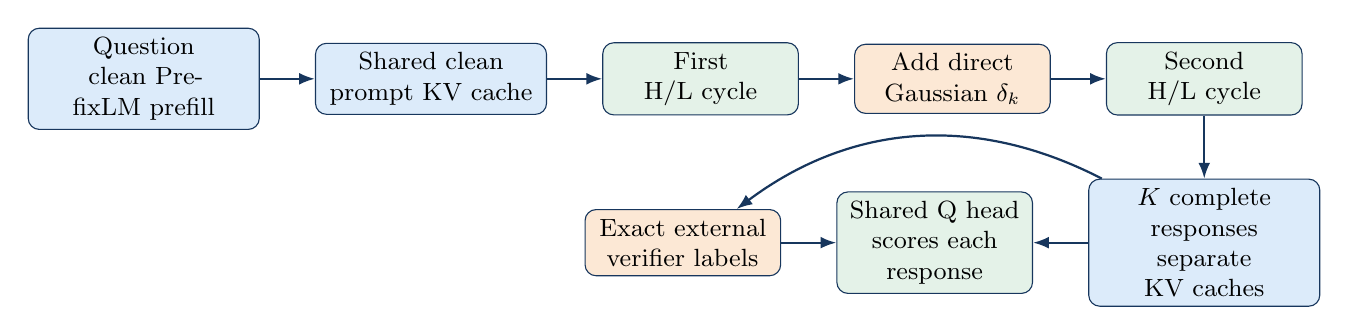
\begin{tikzpicture}[
  node distance=5mm and 7mm,
  box/.style={draw=navy, rounded corners, align=center, minimum height=8mm,
              text width=2.7cm, fill=blue, font=\small},
  smallbox/.style={draw=navy, rounded corners, align=center, minimum height=7mm,
              text width=2.25cm, fill=green, font=\small},
  arrow/.style={-{Latex[length=2mm]}, thick, draw=navy}
]
\node[box] (prompt) {Question\\clean PrefixLM prefill};
\node[box, right=of prompt] (cache) {Shared clean\\prompt KV cache};
\node[smallbox, right=of cache] (h1) {First\\H/L cycle};
\node[smallbox, right=of h1, fill=orange] (adapt) {Add direct\\Gaussian $\delta_k$};
\node[smallbox, right=of adapt] (h2) {Second\\H/L cycle};
\node[box, below=8mm of h2] (answers) {$K$ complete responses\\separate KV caches};
\node[smallbox, left=of answers] (q) {Shared Q head\\scores each response};
\node[smallbox, left=of q, fill=orange] (verify) {Exact external\\verifier labels};
\draw[arrow] (prompt) -- (cache);
\draw[arrow] (cache) -- (h1);
\draw[arrow] (h1) -- (adapt);
\draw[arrow] (adapt) -- (h2);
\draw[arrow] (h2) -- (answers);
\draw[arrow] (answers) -- (q);
\draw[arrow] (answers) to[bend right=32] (verify);
\draw[arrow] (verify) -- (q);
\end{tikzpicture}
\end{center}

\subsection*{The direct Gaussian particle}

The anchor uses $\epsilon_0=0$. Explorer directions are
$\epsilon_k\sim\mathcal{N}(0,I_{1536})$. For H state $h$ and fixed scale
$\alpha$, the parameter-free intervention is
\[
 \delta_k=\alpha\,\operatorname{RMS}(h)
 \frac{\epsilon_k}{\max(\operatorname{RMS}(\epsilon_k),10^{-6})}.
\]
Thus $\operatorname{RMS}(\delta_k)/\operatorname{RMS}(h)\approx\alpha$ and
$\epsilon_0=0$ produces an exactly zero delta. The same direction is reused at
every response step, giving an explorer a coherent trajectory instead of
injecting unrelated token-level noise. There is no learned particle adapter in
the default V1.

The scale is selected once from the predeclared set
$\{0.005,0.01,0.02,0.03,0.05\}$ on 128 unique prompts drawn only from the
training pool. The runner forms deterministic, disjoint 50/50 halves
separately within math and code, interleaving sources before assignment. Scale
zero is a matched control, and every scale uses the same prompts and random
directions. On selection, choose the smallest positive scale within a
predeclared tolerance of the best oracle pass@4; abort if all positive scales
lose to zero. On untouched confirmation, the point-estimate delta versus zero
must be nonnegative overall and separately for math and code. Confirmation
cannot reselect the scale.

The intervention is inserted \textbf{after the first H update and before the
second H/L cycle}.  This matters: the perturbation is processed by another full
reasoning cycle instead of acting as direct noise on the final logits.  Prompt
positions are never perturbed.  Every branch owns a separate KV cache; caches
are not merged.

\subsection*{Making the first sampled token depend on the particle}

HRM-Text expects a bidirectional PrefixLM prompt.  The implementation first
computes that clean prompt once, then appends the fixed causal response prefix
\texttt{\textbackslash nSolution:\textbackslash n}.  Particle injection begins
on those causal prefix tokens.  Thus the first \emph{sampled} answer token can
depend on the particle without changing the official prompt boundary.  All
baselines receive the same fixed prefix.

\subsection*{The Q head}

One shared Q head reads (1) the terminal H2 state for a candidate and (2) the
question summary. It predicts the probability that the response is correct.
The terminal/query states are detached; Q cannot change the frozen generator.
At inference, the chosen response is $\arg\max_k Q(h_T^{(k)},s_x)$.

\newpage
\section*{3. How the proof-of-concept is trained}

This is deliberately a \term{small mechanism test}, not the full research
program.  The 1B HRM backbone, embeddings, and language-model head stay frozen.
The Gaussian intervention has no parameters, so \textbf{only Q is trained} in
the default V1. A later experiment can learn a query-conditioned adapter or add
LoRA, but doing that immediately would make it harder to tell whether gains came
from stochastic H-state search or ordinary parameter adaptation.

\subsection*{Data and verification}

Q warmup collects 2,048 prompt groups---512 each from GSM8K, MATH, DAPO-Math,
and a tested Python set---and generates four candidates per prompt, for 8,192
labelled states.  Prompt groups are source-stratified into 70\% Q training,
10\% epoch selection, 10\% margin selection, and 10\% untouched safety testing.
The default pool contains 2,400 DAPO math prompts and 600 verified Python
prompts (the three-GPU profile uses 4,000 and 1,000) \cite{dapo,openr1}.
Only 128 unique pool prompts are used for the Gaussian scale sweep. Its
selection/confirmation halves are built within each task after deterministic
source interleaving. Training prompts are deduplicated and screened for
13-token overlap with all evaluation prompts; manifests bind exact revisions
and file hashes.

Math is graded by symbolic equivalence.  Generated Python runs only in an
E2B/Morph sandbox through a pinned Open-R1 provider.  A strict harness requires
the candidate to exit normally and match every expected output token; every
remote batch includes a known-good sentinel so an outage cannot silently become
an all-wrong label. Q sees only exact all-tests-pass labels. Fractional test
credit is recorded for analysis and for an optional learned actor, but it does
not change Q's binary target.

\subsection*{Three separated stages}

\begin{enumerate}
  \item \textbf{Scale selection and confirmation.} Compare fixed candidate
  scales with common prompts and random directions. Select the smallest
  positive near-best scale on the selection half; abort if every positive scale
  loses to zero. On confirmation, require a nonnegative point-estimate delta
  overall and within math and code separately. Also set
  \texttt{development\_evidence\_positive} only when the overall paired-bootstrap
  lower bound is above zero. This stronger flag is recorded, not required.
  Save all outcomes, IDs, seeds, rules, and hashes; do not use final benchmarks.
  \item \textbf{Q update.} Verified candidates supervise strict binary
  cross-entropy plus a within-question ranking loss that pushes correct
  candidates above incorrect ones. States are detached. Q's zero-initialized
  last layer and branch-0 tie break preserve the pretrained baseline before Q
  passes a held-out no-degradation gate.
  \item \textbf{Optional learned extension.} In a separate
  \texttt{particles.mode=learned} run, verifier-only PPO may update a bounded,
  query-conditioned adapter. That actor receives leave-one-out correctness and
  anchor-rescue credit; Q still never enters its policy advantage.
\end{enumerate}

\smallnote{\textbf{Non-negotiable rule:} Q is a selector, never the actor's
reward. If a learned extension is run, only the external verifier can reward
the adapter; otherwise it could learn to exploit Q.}

\begin{table}[h]
\small
\centering
\begin{tabular}{ll@{\hspace{1.2cm}}ll}
\toprule
Setting & Primary value & Setting & Primary value \\
\midrule
Particles & $K=4$ & Direction size & 1536 \\
Scale candidates & .005--.05 & Temperature & 0.8 \\
Scale prompts & 128; balanced halves & POC Q states & 8,192 \\
Q learning rate & $3\times10^{-4}$ & Q ranking weight & 0.1 \\
POC train tokens & 256 & POC code-eval tokens & 384 \\
Backbone/particle & frozen / fixed & Q labels & strict binary \\
\bottomrule
\end{tabular}
\end{table}

Gaussian directions are normalized in FP32, scaled relative to each H state's
RMS, then cast to the BF16 activation dtype. Model and Q weights/activations are
BF16; losses, verifier arithmetic, and AdamW master state remain FP32. The
selected-scale and Q artifacts bind the config, model revision, prepared-data
hashes, task-balanced/source-interleaved split IDs, overall/per-task confirmation
gates, stronger confirmation-only evidence flag, RNG seed, and code version.

\newpage
\small
\section*{4. What must be compared}

The primary comparison is \textbf{direct Gaussian particles versus a matched control}
with one clean greedy anchor and three zero-latent samples.  The report also
includes the requested four fully stochastic responses and mathematical
majority vote.  Prompt, prefix, temperature, maximum length, verifier, and
candidate budget stay fixed.  The oracle shows available pass@4 headroom; Q
shows how much can be selected. Q is recalibrated on freshly generated states
from the frozen selected-scale policy, separately for math and code. Ordinary
sampling and Gaussian arms receive identical prompt, prefix, temperature,
maximum length, verifier, and four-response budget.

\section*{5. Evaluation, budget, and decision rule}

Evaluation covers GSM8K, MATH-500, 500 balanced GSM-Symbolic perturbations, and
MBPP+ in a pinned EvalPlus container \cite{evalplus}.  Report anchor accuracy,
mean accuracy, oracle pass@4, math majority vote, Q-selected accuracy, and paired
bootstrap intervals.  GSM-Symbolic resamples original templates rather than
treating correlated variants as independent.  MBPP+ reports base and augmented
pass@1/pass@4 for ordinary, matched, particle, anchor, and Q-selected arms.

\textbf{A promising directional result} should show all of the following:
\begin{itemize}
  \item particle oracle/rescue is higher than matched ordinary sampling, with a
  positive paired confidence interval;
  \item Q-selected accuracy improves over choosing a random candidate and
  captures a useful fraction of oracle headroom;
  \item the anchor remains exact, outputs remain parseable, and length/duplicate
  behavior does not degrade badly;
  \item mixed-outcome groups are common enough to supply useful Q ranking
  signal, and selection captures some of the oracle headroom.
\end{itemize}

The default V1 POC uses two compatible CUDA GPUs and is intended to fit a
roughly 12--15 hour proof-of-concept window including the scale sweep, Q
collection, smoke tests, calibration, and quick evaluation. It is
accelerator-model agnostic: native BF16, NCCL, and sufficient memory are the
requirements. A distributed probe measures a real longest-prompt
rollout/replay/backward and chooses a shared batch near 75\% VRAM with an 80\%
hard cap. Gaussian mode does not spend time on a fake PPO stage: there are no
particle parameters to optimize. The optional learned mode retains a separate
time-boxed actor pilot/run. Provider-side spend limits are still required
because a finished process may leave a rented machine billing.

\subsection*{What this result would---and would not---mean}

A positive POC would show that simple stochastic H-state branching is worth a
larger study; it would not prove that the noise discovers semantic ``reasoning
particles'' or that H-state injection is uniquely better than another control.
A stronger follow-up needs three seeds, private holdouts, $K=1/2/4/8/16$
scaling, a response-start soft-latent control, the learned-adapter mode,
ordinary LoRA RLVR, and Q safeguards against false-positive selection as $K$
grows. If direct Gaussian particles do not beat matched ordinary sampling, the
mechanism has not demonstrated added value, even if outputs look more diverse.

\vspace{-0.4em}
\begin{thebibliography}{9}\small
\bibitem{hrm}
G. Wang et al., ``Hierarchical Reasoning Model,'' arXiv:2506.21734, 2025.
\url{https://arxiv.org/abs/2506.21734}

\bibitem{trm}
A. Jolicoeur-Martineau, ``Less is More: Recursive Reasoning with Tiny
Networks,'' arXiv:2510.04871, 2025.
\url{https://arxiv.org/abs/2510.04871}

\bibitem{ptrm}
A. Sghaier, A. Parviz, and A. Jolicoeur-Martineau, ``Probabilistic Tiny
Recursive Model,'' arXiv:2605.19943, 2026.
\url{https://arxiv.org/abs/2605.19943}

\bibitem{hrmtext}
G. Wang et al., ``HRM-Text: Efficient Pretraining Beyond Scaling,''
arXiv:2605.20613, 2026.
\url{https://arxiv.org/abs/2605.20613}

\bibitem{modelcard}
Sapient Intelligence, ``HRM-Text-1B Model Card,'' 2026.
\url{https://huggingface.co/sapientinc/HRM-Text-1B}

\bibitem{dapo}
Open-R1, ``DAPO-Math-17k-Processed.''
\url{https://huggingface.co/datasets/open-r1/DAPO-Math-17k-Processed}

\bibitem{openr1}
Hugging Face, ``Open-R1.''
\url{https://github.com/huggingface/open-r1}

\bibitem{evalplus}
EvalPlus, ``Rigorous Evaluation of LLM-Synthesized Code.''
\url{https://github.com/evalplus/evalplus}
\end{thebibliography}

\end{document}
